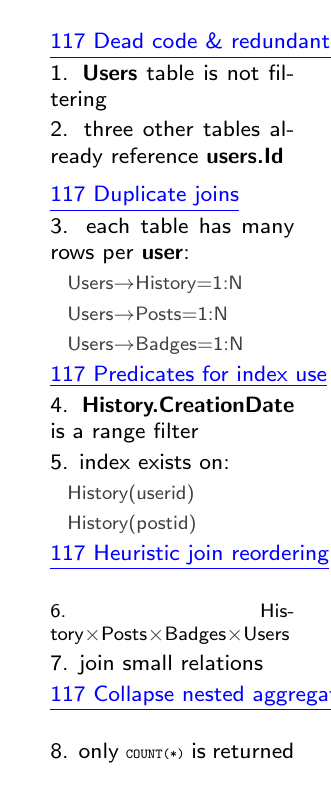
\begin{tikzpicture}[node distance=5pt,font=\small, line width=.5pt, inner sep=0mm,
    tablestyle/.style={draw=none, fill=none, inner sep=0, outer sep=0pt},shape=rectangle,align=center]


    \sffamily
    \node [tablestyle] (r) {
      \setlength{\tabcolsep}{0pt}
      \hspace{2pt}
      \begin{tabular}{p{3.1cm}}          
          \footnotesize{\textcolor{blue}{\underline{\ding{117} Dead code \& redundant ops}}} \\ %\chline 
          \footnotesize{1. \textbf{Users} table is not filtering } \\   
          \footnotesize{2. three other tables already reference \textbf{users.Id}} \vspace{3pt}\\  
          %
          \footnotesize{\textcolor{blue}{\underline{\ding{117} Duplicate joins}}} \\ %\chline     
          \footnotesize{3. each table has many rows per \textbf{user}:} \\
          \ \ \scriptsize{\textcolor{darkgray}{Users$\rightarrow$History=1:N}}\\
          \ \ \scriptsize{\textcolor{darkgray}{Users$\rightarrow$Posts=1:N}}\\
          \ \ \scriptsize{\textcolor{darkgray}{Users$\rightarrow$Badges=1:N}} \vspace{0.3pt}\\ %\chline  
          %
          \footnotesize{\textcolor{blue}{\underline{\ding{117} Predicates for index use}}} \\ %\chline 
          \footnotesize{4. \textbf{History.CreationDate} is a range filter} \\
          \footnotesize{5. index exists on:} \\ 
          \ \ \scriptsize{\textcolor{darkgray}{History(userid)}}\\ 
          \ \ \scriptsize{\textcolor{darkgray}{History(postid)}}\\ 
          %
          \footnotesize{\textcolor{blue}{\underline{\ding{117} Heuristic join reordering}}} \vspace{0.3pt}\\  
          \scriptsize{6. History\textcolor{darkgray}{$\times$}Posts\textcolor{darkgray}{$\times$}Badges\textcolor{darkgray}{$\times$}Users} \\
          \footnotesize{7. join small relations} \\
          %
          \footnotesize{\textcolor{blue}{\underline{\ding{117} Collapse nested aggregates}}} \vspace{0.3pt}\\ 
          \footnotesize{8. only \tiny{\texttt{COUNT(*)}}\footnotesize\ is returned}
        \end{tabular}
    };
   %\draw [black,rounded corners=.3em, fill=lightgray!60, opacity=0.1] (r.north west) rectangle (r.south east);

% * (5) Dead code & redundant operations
%         - users table is not filtering anything
%         - All joins are via:
%             Badges.UserId
%             PostHistory.UserId
%             Posts.OwnerUserId
%         - These columns are already foreign keys to Users.Id

% * (6) Duplicate joins & row explosion
%         - Each table has many rows per user:
%             Users → History = 1:N
%             Users → Posts = 1:N
%             Users → Badges = 1:N
%         - Why this is messy
%             The original query joins three N-side tables simultaneously:
%             User → History × Posts × Badges
% * (8) Predicates for optimal index usage
%     History.CreationDate:
%     timestamp without time zone

%     Index exists on:
%         History(userid)
%         History(postid)
%     Query filters on CreationDate range
%     Why original query is inefficient
%     Filter applied after multi-table join
%     Prevents early row elimination
%     Index on CreationDate (if present or composite) is underutilized  
% * (14) Heuristic join reordering
% ---------------------------
% Evidence
% Table	Rows	Notes
% History	303k	Time-filtered
% Posts	92k	PostTypeId highly selective
% Badges	80k	Unfiltered
% Why original plan is bad

% Planner must consider:

% History × Posts × Badges × Users


% Large search space with poor early selectivity.

% Why rewrite is better

% You manually enforce:

% Filter

% Aggregate

% Join small relations

% Each CTE collapses to ≈ number of users, not rows.
% --------------------

% * (16) Collapse nested aggregates
% Metadata-based reason
% Evidence

% Each table has multiple rows per user

% Only final output is COUNT(*)

% Why original aggregation is expensive

% COUNT runs over a huge Cartesian join

% Every duplicate combination is materialized
% ----------------------------------------------
% CTE optimization
% Metadata-based reason
% Evidence

% Each CTE reduces:

% 80k–300k rows
% → ~10k users (approx.)

% Why CTEs make sense here

% Logical isolation per table

% Clear cardinality reduction

% Prevents accidental re-expansion

% In PostgreSQL ≥12:

% CTEs are inlineable

% No performance penalty

% ✔ Label_21 justified by strong row reduction

% ---------------------------------------



%    * Redundancy & Efficiency:
%             Label_5: Dead code & redundant operations
%             Label_6: Unused columns, and duplicate predicates/joints
%             Label_7: Simplify DISTINCT clauses and unnecessary nesting

%         * Access & Sargability
%             Label_8: Predicates for optimal index usage
%             Label_9: Functions-on-columns to range predicates
%             Label_10: Recommend expression/partial indexes
%             Label_11: Replace LIKE '%x' with trigram/full-text patterns
%             Label_12: Normalize types to avoid casts
%             Label_13:Trim SELECT * to needed columns

%         * Join Logic:
%             Label_14: Heuristic join reordering
%             Label_15: Change join types

%         * Aggregation & Windowing:
%             Label_16: Collapse nested aggregates/windows
%             Label_17: Replace DISTINCT-on-join
%             Label_18: Remove unnecessary PARTITION/ORDER

%         * Subquery & CTE Optimization:
%             Label_19: Scalar subqueries
%             Label_20: Transform IN/NOT IN to EXISTS/NOT EXISTS
%             Label_21: Inline CTEs or mark MATERIALIZED

   
\end{tikzpicture}
